\chapter{A Mystery Square Circle}
The cover shown in Figure~\ref{delagoa} is a bit of a mystery. The cover originally was in the collection of Harry Birkhead which was dispersed in 2014 by Spinks of London. The cover bears a Transvaal stamp and was tied by a Cape Town squared-circled datestamp and addressed to London. As the envelope is addressed to London and presumably posted in Cape Town it does not make sense to bear a Transvaal stamp. 

\begin{figure*}
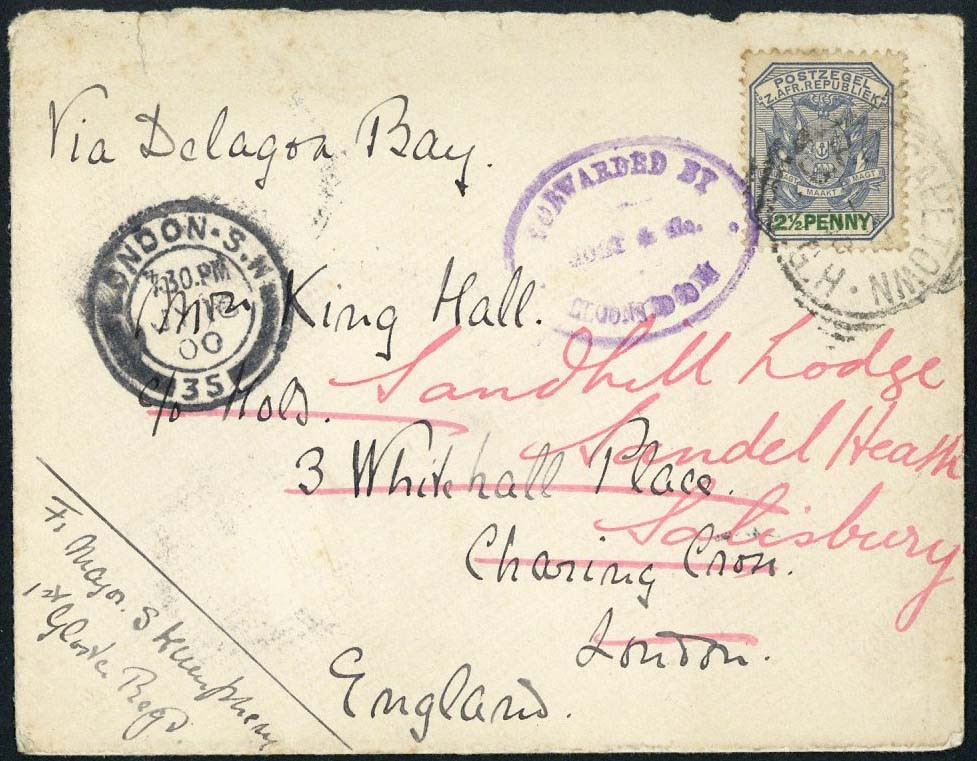
\includegraphics[width=1.0\textwidth]{../cape-of-good-hope/14018_89_1.jpg}
\caption{
Lot: 89 (x) British Forces Mail
1900 (27 June) envelope (part flap missing) from a Major in the 1st. Gloucester Regiment "Via Delagoa Bay" to London, bearing Transvaal 2½d blue and green tied by Cape Town squared-circle datestamp, upon arrival redirected to Salisbury with London c.d.s. (12.7) and oval-framed "forwarded by/holt & co/london" cachet in violet; unusual 
Estimate  \pound80 to  \pound100}\label{delagoa}
\end{figure*}

Another peculiarity was that the envelope was marked via Delagoa Bay in Mozambique, which would be the quickest shipping route from the Transvaal. This route during 1900 would have not been very safe in as the Boer commandos were still active in these areas. It is probable that due to the difficulties of this route the envelope was routed via Cape Town and was stamped in the G.P.O. without attracting tax. It then found its way to London and the rest of the story is not difficult to follow. 

